\documentclass[conference]{IEEEtran}
\IEEEoverridecommandlockouts
% The preceding line is only needed to identify funding in the first footnote. If that is unneeded, please comment it out.
\usepackage{cite}
\usepackage{amsmath,amssymb,amsfonts}
\usepackage{graphicx}
\usepackage{textcomp}
\usepackage{xcolor}
\usepackage{subfig}
\usepackage{algorithm}
\usepackage{algpseudocode}
\usepackage{diagbox}
\usepackage{footnote}
\usepackage{bbding} %\Checkmark \XSolid
% to be able to draw some self-contained figs
\usepackage{tikz}
% inlined bib file
\usepackage{filecontents}

\def\BibTeX{{\rm B\kern-.05em{\sc i\kern-.025em b}\kern-.08em
    T\kern-.1667em\lower.7ex\hbox{E}\kern-.125emX}}
\begin{document}

\title{Dynamic Lock Violation for Fault-tolerant Distributed Database System}


\author{\IEEEauthorblockN{Hua Guo}
\IEEEauthorblockA{\textit{School of Information} \\
\textit{Renmin University of China}\\
Beijing, China \\
guohua2016@ruc.edu.cn}
\and
\IEEEauthorblockN{Xuan Zhou}
\IEEEauthorblockA{\textit{School of Data Science And Engineering} \\
\textit{East China Normal University}\\
Shanghai, China \\
xzhou@dase.ecnu.edu.cn}
}

\maketitle

\begin{abstract}
Modern distributed database systems scale horizontally by sharding its data on a large number of nodes.
To achieve fault tolerance, most of such systems build their transactional layers on a replication layer,
which employs a consensus protocol to ensure data consistency.
Synchronization among replicated state machines thus becomes a major overhead of transaction processing.
Without a careful design, synchronization could amplify transactions' lock duration and impair the system's scalability.
Speculative techniques, such as Controlled Lock Violation (CLV) and Early Lock Release (ELR), prove to be effective in shortening lock duration and boosting performance of transaction processing.
An intuitive idea is to use these techniques to optimize geo-replicated distributed databases.
In this paper, we show that direct application of speculation is often unhelpful in a distributed environment.
Instead, we introduce Dynamic Lock Violation (DLV), a speculative technique for geo-replicated distributed databases.
DLV chooses the right time to conduct lock violation, so that it can achieve good performance without incurring severe side effects.
\end{abstract}

\begin{IEEEkeywords}
Database System, Distributed Transaction, Locking, High Availability
\end{IEEEkeywords}

\section{Introduction}

Modern distributed database system scale out by partitioning data across multiple nodes, so that it can run transactions on multiple servers in parallel to increase throughput.
When a transaction needs to access multiple partitions, it has to employ a coordination protocol to ensure atomicity.
It is commonly known that such distributed transactions can lead to significant performance degradation.
This is mainly due to the following reasons\cite{Calvin:conf/sigmod/ThomsonDWRSA12}:

1. Coordinated commit requires a chatty protocol (e.g., Two-Phase Commit), which introduces tremendous network overheads;

2. Message transmission overlaps with the critical path of transaction commit, which worsens the contention among transactions.

These issues can be more serious for geo-replicated databases, which face increased network overheads.
%Transactional layer uses a specific concurrency control(CC) scheme to enforce a serializable schedule and a distributed commit protocol if transaction access multiple shards.
%Optimistic CC scales well when there is little contention but suffers high abort rate when it dealing with a workload of high degrees of contention.
%Pessimistic CC has a lower abort rate, but it endures overheads of blocking.
%In fact, CC matters little on performance if no conflicts and no most CC schemes failed to handle high contention\cite{PerformanceOfCC:conf/vldb/CareyS84}\cite{EvaluationOfCC:journals/pvldb/HardingAPS17}.
The replication layer of a geo-replicated database often uses a Paxos-like consensus protocol to ensure consistency among replicas.
This introduces a significant amount of message transmission, which further increase the duration of transactions.
To facilitate replication, we usually split data into small chunks and replicate each chunk independently.
As a result, cross-chunk transactions (rather than cross-partition transactions) all become distributed transactions.
This makes distributed transaction even more inevitable.

\begin{figure}[htbp]
  \centerline{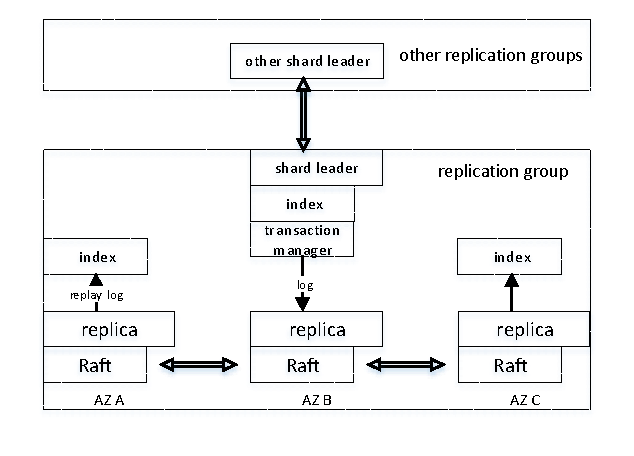
\includegraphics[scale=0.8]{figure/architecture.pdf}}
  \caption{Typical architecture of geo-replicated distributed DBMS}
  \label{fig:architecture}
\end{figure}

Figure~\ref{fig:architecture} presents the typical architecture of geo-replicated distributed databases.
The database partitions its data into a number chunks.
For each chunk, the replication layer replicates its data to several Availability Zones (AZ) \cite{Aurora:conf/sigmod/VerbitskiGSCGBM18}.
Among the available zones, the replication layer employ a consensus protocol to shield data consistency.

As previous work has discussed \cite{Calvin:conf/sigmod/ThomsonDWRSA12}\cite{Tapir:conf/sosp/ZhangSSKP15}\cite{Janus:conf/osdi/MuNLL16},
this architecture has to rely on a chatty protocol (which integrates the commit protocol and the consensus protocol) to ensure the correctness of transactions.
It may fail to scale when confronted with highly contended workload.
Nevertheless, this architecture supports a wide range of transaction processing methods.
Most industrial data systems choose this two-layer architecture, including Google Spanner \cite{Spanner:conf/osdi/CorbettDEFFFGGHHHKKLLMMNQRRSSTWW12}\cite{Spanner:conf/sigmod/BaconBBCDFFGJKL17},
NuoDB \cite{NuoDB}, CockroachDB \cite{CockroachDB}, TiDB \cite{TiDB}, etc.

\begin{figure}[htbp]
  \centerline{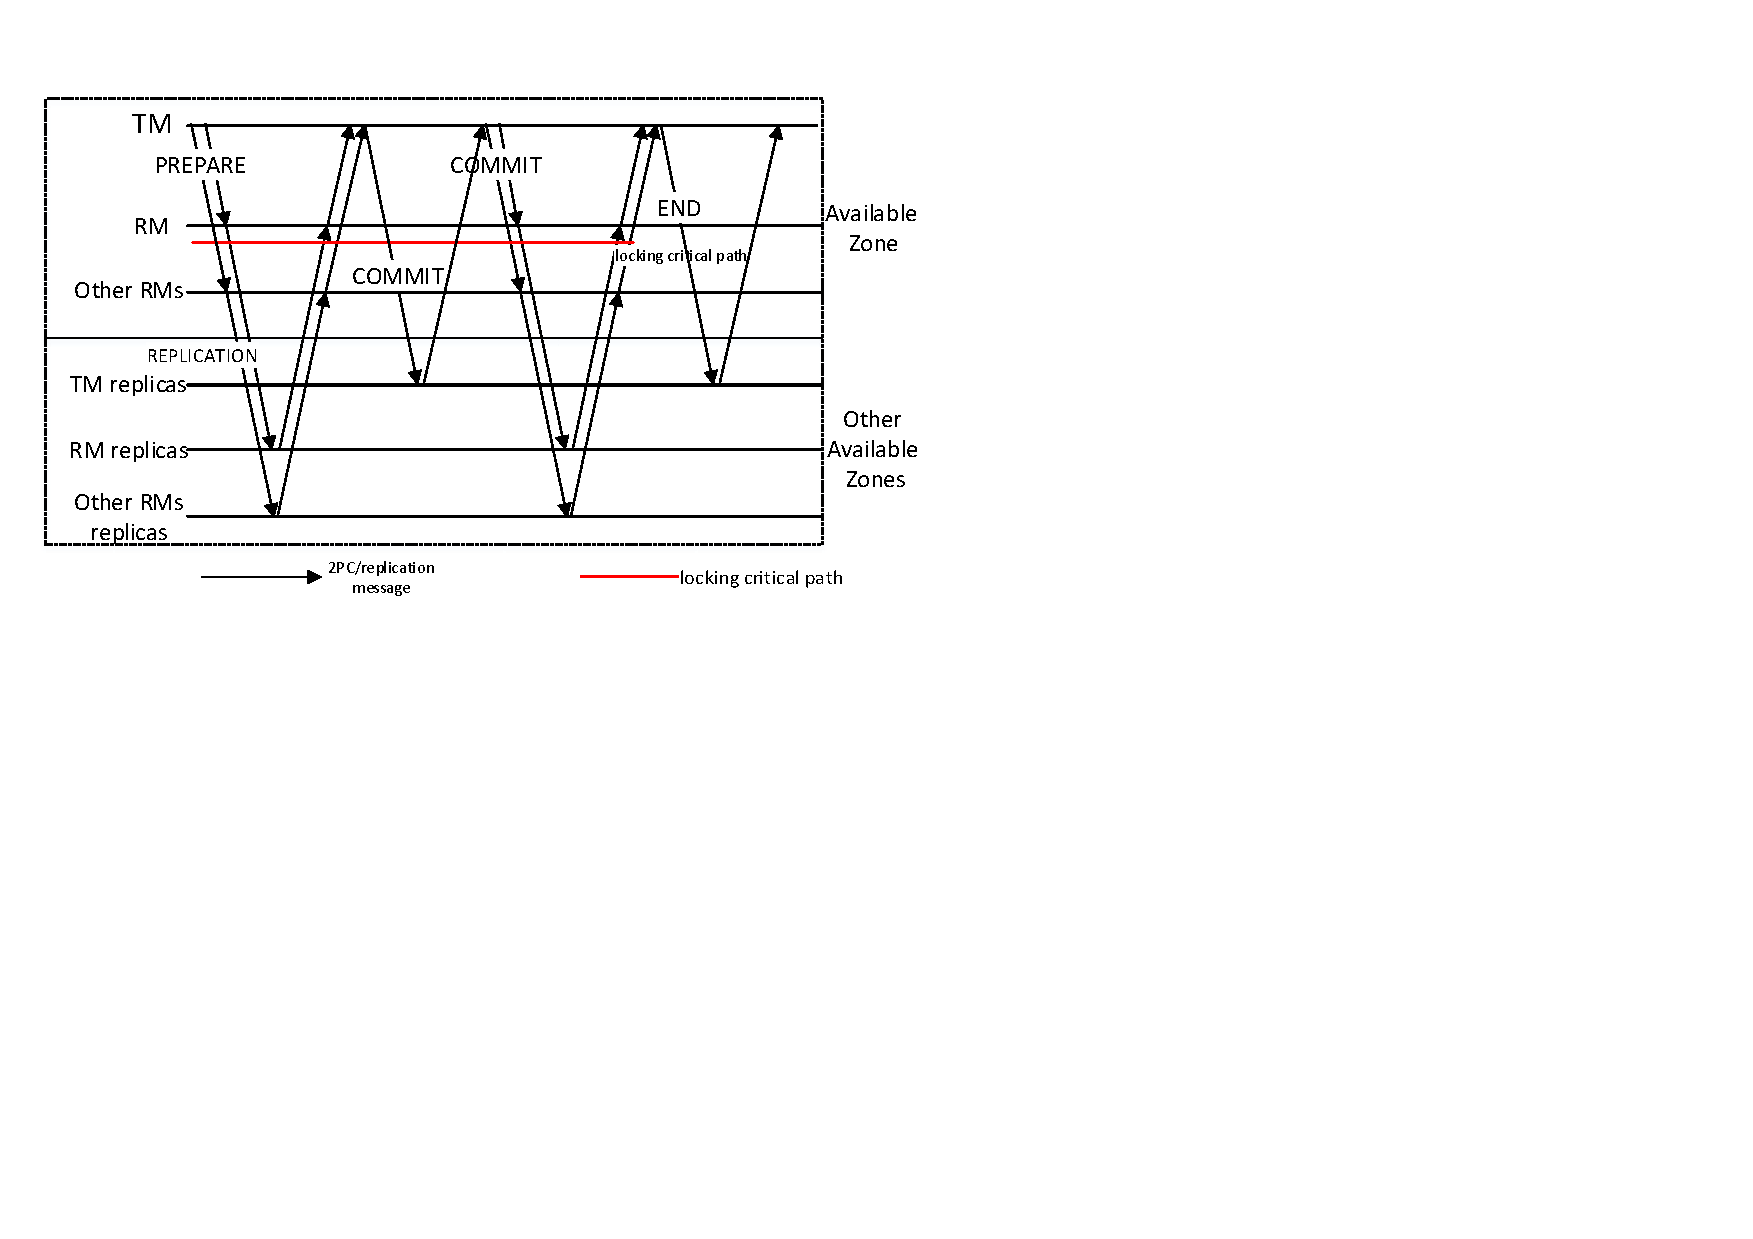
\includegraphics[scale=0.62]{figure/message_flow.pdf}}
  \caption{The message flow and lock holding critical path when the DBMS uses S2PL for concurrency control and 2PC as the commit protocol.
The dash arrow lines represents the messages introduced by Dynamic Lock Violation (DLV). The red lines represent the critical paths of S2PL.
The green dash lines represent the critical paths of DLV.}
  \label{fig:two_layers_architecture}
\end{figure}

Looking more closely, the main issue is that the commit and consensus protocols enlarge the timespan of the critical paths in transaction processing.
This significantly amplifies the overhead of contention.
%We focus on distributed DBMS which uses locking scheme and coordination protocol on a replicated layer, especially who running transaction processing on geo-replicated layer.
Figure \ref{fig:two_layers_architecture} shows the message flow of a distributed transaction in such an architecture. We assume that
it uses S2PL for concurrency control and 2PC as the commit protocol, and the replication layer is deployed over a WAN.
When a transaction requests to commit, the \emph{TM (transaction manager)} issues a `prepare' message to each \emph{RM (resource manager)}.
Then, each \emph{RM} replicates its vote (`prepare commit' or `prepare abort') to the corresponding replicas through a consensus protocol, before it
sends its vote to \emph{TM}.
After the \emph{TM} collects all the votes of the \emph{RMs},
it broadcasts the final decision (`commit' or `abort') to all the \emph{RMs}
\footnote{Depending on variants of implementations, the TM can choose to persist its decision on its log or not.}
.
Once a \emph{RM} receives the final decision from the \emph{TM}, it replicates the decision to the corresponding replicas.
After the consensus of commit or abort is reached, the \emph{RM}
can release the locks that it had retained over the accessed data.

We depict lock duration by red lines in Figure~\ref{fig:two_layers_architecture}.
As we can see, the lock duration span multiple message round trips, including those over the WAN.
This will severely impair the concurrency of transaction processing in face of a high degree of contention.

Speculative techniques, such as Early Lock Release (ELR) \cite{EfficientLocking:conf/vldb/KimuraGK12} and Controlled Lock Violation (CLV)
\cite{CLV:conf/sigmod/GraefeLKTV13}, prove to be effective in optimizing centralized transaction processing.
These techniques can be extended to a distributed environment.
%The two-layer architecture shares the same bottleneck with single node DBMS on forcing transaction log and faces even worse conditions.
%Figure \ref{fig:log_write_latency} shows the log write latency of different environment(TODO... experiments setting).

\begin{figure}[htbp]
  \centerline{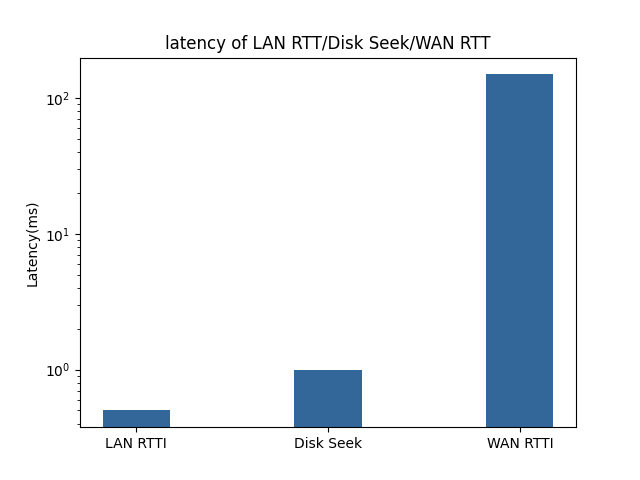
\includegraphics[scale=0.4]{figure/log_write_latency.png}}
  \caption{log write latency in different environment}
  \label{fig:log_write_latency}
\end{figure}

Speculative techniques improve concurrency by excluding logging from lock duration,
Transactions on geo-replicated distributed databases require much more time to ship and persist logs.
This provides more opportunities for exploiting speculation.
However, application of speculation in a distributed environment is complex.
A number of design choices need to be considered.
For instance, when working with 2PC, we need to decide to violate (or release) lock at which phase.
As previous work showed \cite{CLV:conf/sigmod/GraefeLKTV13}, lock violation at the first phase may enable a higher degree of concurrency.
However, dependency tracing and cascade abort may incur excessive overheads.
On the contrary, lock violation at the second phase costs less in dependency tracing and cascade abort, while it has to sacrifice a certain amount of concurrency.
%Transaction models, interactive or one-shot transactions, may have different message flow, how different transaction types could benefit from these techniques?
On the other hand, not all transactions can benefit from CLV or ELR, e.g., workload with little conflict.
It unnecessary and even harmful to apply speculation to all cases.

In this paper, we propose a technique called Dynamic Lock Violation (DLV) to enhance the performance of geo-replicated distributed DBMS.
DLV decides the best time to perform lock violation by looking at runtime statistic information.
It introduces much less penalty compared to previous implementation \cite{CLV:conf/sigmod/GraefeLKTV13}.

The remainder of this paper is organized as follows.
Section \ref{sec:relate_work} reviews related work.
Section \ref{sec:non_strict} shows that a strict schedule is not necessary and hurt the performance of distributed DBMS.
Section \ref{sec:implement} introduces DLV.
Section \ref{sec:experiments} evaluates DLV and compare it against previous work.
Section \ref{sec:conclution} concludes this paper.


\section{Relate Work}
\label{sec:relate_work}
%This section introduces the related work of this paper.

\subsection{Transaction Processing on Replicated Databases}
%Recently, there are many scalable DBMS arisen in both academia and industry.
%Most of the systems in this category supports distributed query processing and
%replicate data across several data center geo-located in different areas for fault tolerance.

Most replicated databases rely on state-machine replication(SMR) to realize high availability.
SMR often uses a consensus protocol to synchronize different replicas.
Synchronization introduces significant amount of network traffic and becomes a major overhead of replicated database systems.
Paxos \cite{Paxos:journals/tocs/Lamport98}\cite{PaxosSimple:conf/opodis/Lamport02} is the most well known consensus protocol.
To reach a consensus on a single data update in Paxos, it costs two message round trips, one for choosing a proposal and another for proposing the entry.
Multidecree Paxos\cite{Multidecree:journals/csur/RenesseA15} elects a leader as the only proposer to eliminate the first message round trip.
Raft\cite{Raft:conf/usenix/OngaroO14} is a similar consensus protocol to Paxos. As it is more understandable, it is widely used in modern database systems.
In Raft, it costs at least one message round trip to reach a consensus.
Google Spanner \cite{Spanner:conf/osdi/CorbettDEFFFGGHHHKKLLMMNQRRSSTWW12}\cite{Spanner:conf/sigmod/BaconBBCDFFGJKL17},
NuoDB \cite{NuoDB}, CockroachDB \cite{CockroachDB} and TiDB \cite{TiDB} are all geo-replicated DBMSes built upon Paxos or Raft.
They all face heavy costs incurred by data synchronization.

To minimize the cost of synchronization, a number of techniques have also been proposed.
VoltDB \cite{VoltDB} and Calvin \cite{Calvin:conf/sigmod/ThomsonDWRSA12} employ a deterministic transaction model
to reduce the coordination cost of distributed transactions.
Deterministic scheduling enables active replication, which allows transactions to kickoff synchronization at the earliest possible time.
Tapir \cite{Tapir:conf/sosp/ZhangSSKP15} relaxes the consistency requirements of the replication layer, so that it can reduce the message round trips to reach consensus.
Janus \cite{Janus:conf/osdi/MuNLL16} aims to minimize wide-area message round trips
by consolidating the concurrency control mechanism and the consensus protocol.
It uses deterministic serializable graph tracing to ensure atomicity of transactions.
In a nutshell, Tapir and Janus both co-designed the transaction and replication layers of distributed databases, so that they only need to incur one wide-area message round trip to commit a transaction.
VoltDB, Calvin, Tapir and Janus all impose strict constraints on the implementation of the transaction layer, making them incompatible with existing systems, such as Spanner and CockroachDB.
In contrast, this work focuses on the optimization opportunities in the general implementation of geo-replicated databases (as depicted in Figure~\ref{fig:architecture}).

\subsection{Optimization on Locking based Concurrency Control}
%DBMS use concurrency control(CC) to calculate a serializable schedule for concurrent transactions.
Two-phase locking (2PL) is the most widely used concurrency control mechanism.
As a pessimistic method, 2PL assumes a high likelihood of transaction confliction.
It uses locks to enforce the order of conflicting transactions.
Strict 2PL (S2PL) is a brute force implementation of 2PL. 
It requires a transaction to preserve all its lock until it ends.
As S2PL can easily guarantee transactions' recoverability, many databases choose to use it.
When extending S2PL to distributed databases, the lock holding time will be substantially enlarged, 
as the commit critical path will involve a number of message round trips.

All S2PL implementations adopt a certain approach to resolve deadlocks.
In the \emph{no-wait}
\cite{EvaluationOfCC:journals/pvldb/HardingAPS17}
approach, a transaction immediately aborts if it fails to place a lock.
Previous works showed that this is a scalable approach in a distributed environment \cite{EvaluationCC1000Cores:journals/pvldb/YuBPDS14}\cite{EvaluationOfCC:journals/pvldb/HardingAPS17},
as it eliminates blocking completely.
However, it works poorly when dealing with workload of high contention.
Another approach is \emph{wait-die} \cite{LockNoWait:journals/csur/BernsteinG81}. 
It avoids some false-positive aborts encountered by \emph{no-wait} by utilizing timestamps.
The \emph{Deadlock detection} approach \cite{LockCC:conf/ds/GrayLPT76} detects deadlock by explicitly tracing wait-for relationship among transactions.
Many centralized database systems \cite{MySQL}\cite{PostgreSQL} adopt this approach, as can deal with contention better.
However, deadlock detection in a distributed environment is highly costly, making it the least favorable approach in our case.

%\subsection{Exploit Speculation and Lock Violation}
To optimize the performance of locking based concurrency control, speculation can be used.
%Similar approaches have been introduced by many previous works.
Early lock release (ELR)
\cite{ELR:dewitt_implementation_1984}\cite{PS2PL:conf/icdt/Soisalon-SoininenY95}
\cite{Aether:journals/pvldb/JohnsonPSAA10}
\cite{EfficientLocking:conf/vldb/KimuraGK12}
\cite{Actor-Oriented-DB:conf/icde/Bernstein18}
is a typical speculative technique.
ELR allows a transaction to release its locks before its commit log is flushed to disk.
It was first proposed by DeWitt et al.\cite{ELR:dewitt_implementation_1984}.
Soisalon-Soininen et al.\cite{PS2PL:conf/icdt/Soisalon-SoininenY95} analyzed its correctness in various settings.
Many other works applied and evaluated ELR in different types of systems \cite{Aether:journals/pvldb/JohnsonPSAA10}\cite{EfficientLocking:conf/vldb/KimuraGK12}\cite{EfficientLocking:conf/vldb/KimuraGK12}\cite{Aether:journals/pvldb/JohnsonPSAA10}.
However, previous works on ELR were limited to centralized database systems.
%Jones et al.\cite{LowOverheadCC:conf/sigmod/JonesAM10} use a restirct transaction model\cite{H-store:journals/pvldb/KallmanKNPRZJMSZHA08} implement sepculation.

Control lock violation (CLV) \cite{CLV:conf/sigmod/GraefeLKTV13} is a more general speculative technique than ELR.
It allows certain transactions to ignore certain locks, instead of releasing a lock completely.
CLV has been tested on distributed databases. The results show that it can optimize both phases of two-phase commit.
CLV needs to trace dependency among transactions.
In \cite{CLV:conf/sigmod/GraefeLKTV13}, the authors use a Register and Report (RARA) approach \cite{HeckatonMVCC:journals/pvldb/LarsonBDFPZ11} to implement the tracer.
RARA work well on a centralized database. In a distributed environment, dependency tracing becomes much more costly.
Cascade abort is another side effect of speculation. It can also leads to severe performance downgrade for distributed databases.


\section{Scheduling with Lock Violation}
\label{sec:non_strict}

In the following, we describe how to ensure correct scheduling with lock violation.

\subsection{Preliminaries and Assumptions}
A database system normally shards its data by primary keys.
For each data chunk, we replicate its physiological logs across different AZs to achieve fault-tolerance.
The physiological logs record the row-level write operations of each transaction.
The replicated layer uses consensus protocol to maintain the consistency among the replicas.
%Other replication protocols may also work.
We assume that there is a replica leader for each data chunk, which is responsible for receiving requests.

We assume that the system supports both one-shot and interactive transactions.
Figure \ref{fig:transaction_type} shows the message flow during the commit phase of the two types of transaction.
We can see that an interactive transaction costs more message round trips than a one-shot transaction.
%These two types of transaction model employ different message flow.
Our lock violation technique must work with both types of transactions, which we will explain subsequently.

\begin{figure}[htbp]
    \centering
    \captionsetup[subfigure]{oneside,margin={0.3cm,0cm}}
    \subfloat[one-shot transaction, the prepare message is a suggestive one to let the RM issue response commit/abort message ]
        { 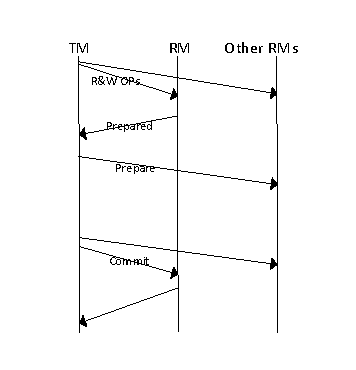
\includegraphics[scale=1] {figure/transaction_oneshot}  \label{fig:transaction_oneshot}  }
    \captionsetup[subfigure]{oneside,margin={0.3cm,0cm}}
    \subfloat[interactive transaction, when a RM receive a \emph{Prepare} message, transaction can prevent deterministic abort. ]
        { 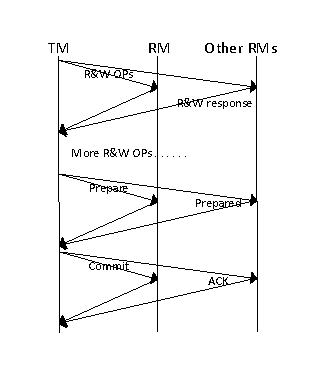
\includegraphics[scale=1]{figure/transaction_interactive} \label{fig:transaction_interactive}}

  \caption{commit message flow of one-shot and interactive distributed transaction}
  \label{fig:transaction_type}
\end{figure}



\subsection{Concepts of Scheduling}
Before presenting our method, we first review the conceptual model of transaction processing. Most of the contents can be found in the previous work \cite{LockNoWait:journals/csur/BernsteinG81}.

\subsubsection{Transaction and History}
Suppose a distributed database resides on ${n}$ nodes, represented by ${R = \{r_1, r_2, ... r_n\}}$.
A transaction ${T_i}$ can run on any ${m}$ of the ${n}$ nodes ($1 \le m \le n$), represented by  ${S = \{s_1, s_2, ... s_m\} \subseteq R}$, 
The transaction ${T_i}$ is composed of a series of operations, %, represented by ${O = \{o_1, o_2, ... o_k\}}$. 
%Each $o_i \in O$ 
where each operation can be a read or a write or any command operation including abort, commit, etc.
Let ${r_i[x]}$ denote that ${T_i}$ reads record ${x}$,  and ${w_i[x]}$ denotes that ${T_i}$ writes record ${x}$.
Let ${c_i}$, ${a_i}$, ${p^c_i}$, ${p^a_i}$ denote the commit, abort, prepare-to-commit and prepare-to-abort operations of ${T_i}$ respectively.
We call ${T_i}$'s operations on the node ${s_u}$ ${T_i}$'s \emph{sub-transaction} on ${s_u}$.
A transaction history is a collection ${H = \{h_1, h_2, ..., h_n\}}$, in which
each ${h_u}$ is the local history of $H$ on the node ${s_u}$, which is a sequence of operations issued by different transactions.

%in which ${h_u (1 \le u \le n) = \Pi_u(H)}$ is the local history on site ${s_u}$.
%${\Pi_u(H)}$ is ${H}$'s projection on site ${s_u}$.
%For any projected history ${h_u(1 \le u \le m)}$, ${h_{u} }$ is a collection of  operations requests by many transactions.

\subsubsection{Deterministic and Non-deterministic Abort}
A number of reasons can cause a transaction to abort. In general, they can be categorized as:

1. User requested abort. These are aborts specified by the program logic (e.g., requiring a transaction to abort if it has accessed non-existent records);

2. Violation of isolation (e.g., serializability);

3. Database node failure. For simplicity, we assume fail-stop failures only.

We call the first two types of abort \emph{deterministic abort} and the last one \emph{non-deterministic abort}, 
as the latter is not predictable using the operational logic of the database system.

\subsubsection{Dependencies among Transaction}

There are there kinds of data dependency among transactions, known as \emph{wr-dependency}, \emph{ww-dependency} and \emph{rw-dependency}.
In a local history ${h}$, if ${T_j}$ reads ${T_i}$'s write on ${x}$,
we call it a \emph{write-after-read(wr) dependency} and denote it by ${w_i[x] \rightarrow r_j[x]}$.
Analogically, if ${T_j}$ overwrites ${T_i}$'s write on ${x}$, it is \emph{write-after-write(ww) dependency} and denoted by ${w_i[x] \rightarrow w_j[x]}$.
If ${T_i}$ reads ${x}$ before ${T_j}$ writes on ${x}$, it is a \emph{read-after-write(rw) dependency} and denoted by ${r_i[x] \rightarrow w_j[x]}$.

Based on data dependencies, we can define \emph{commit dependency}. ${T_j}$ has a \emph{commit dependency} on ${T_i}$, written as ${T_i \rightarrow T_j}$, if ${T_j}$ cannot commit prior to ${T_i}$.
In other words, ${T_i}$ aborts, ${T_j}$ has to abort too. ${T_j}$ has a \emph{commit dependency} on ${T_i}$, if and only if ${T_j}$ has a \emph{rw-dependency} or \emph{ww-dependency} on ${T_i}$.

A transaction ${T_j}$ \emph{speculatively access} a record ${x}$, if there is another transaction ${T_i}$,
${T_j}$ has a commit dependency on ${T_i}$ and  ${T_i}$ has not committed.
We call such a commit dependency a \emph{danger dependency}, denote it as ${T_j \rightarrow_s T_i}$.

\subsubsection{Relaxation on Strictness}

Traditional transaction schedulers choose strict two-phase locking (S2PL) \cite{DBLP:conf/vldb/Raz92} to avoid expensive transaction recovery cost.
Strictness implies that a transaction cannot read or overwrite a previous write by another transaction which has not committed yet.
%For a locking base concurrency control scheme, the lock will hold until the transaction end, namely strict two-phase locking(S2PL).

Strictness is not a necessary condition for a correct schedule.
%\subsection{Strict Scheduler is Too ``Strict" for Correctness}
For instance, the schedule ${H_1}$ of Figure \ref{fig:strict_example} is serializable and strict. %there are 3 working nodes, ${s_1}$, ${s_2}$, ${s_3}$.
(The data dependencies include ${r_1[x] \rightarrow w_3[x]}$, ${w_1[x] \rightarrow r_2[y]}$, ${r_2[y] \rightarrow w_3[x]}$.) 
In contrast, ${H_2}$ in Figure~\ref{fig:non_strict_example} is serializable but not strict.
In Figure~\ref{fig:non_strict_example}, there are three records ${x}$, ${y}$, ${z}$, residing on ${s_1}$, ${s_2}$, ${s_3}$ respectively.
${T_1}$ writes ${y}$ and ${x}$.
${T_2}$ reads ${T_1}$'s write on ${x}$ before ${T_1}$ commits.
Transaction ${T_3}$ overwrites ${T_2}$'s write before ${T_2}$ commits.
The schedule ${H_2}$ can be represented as
\begin{center}
  ${H_2 = \{h_1, h_2, h_3\}}$,
\end{center}
in which,
\begin{center}
${h_1=w_1[x], w_3[x], p^c_1, c_1, p^c_3, c_3}$

${h_2=w_1[y], r_2[y], p^c_1, c_1, p^c_2, c_2}$

${h_3=r_2[z], w_3[z], p^c_2, c_2, p^c_3, c_3 }$.
\end{center}


%Both of ${H_1}$ and ${H_2}$ are serializable equal with the serial schedule, ${T_1}$ ${T_2}$ ${T_3}$.
%Scheule ${H_1}$ and ${H_2}$ are correct.


\begin{figure}[htbp]
  \centerline{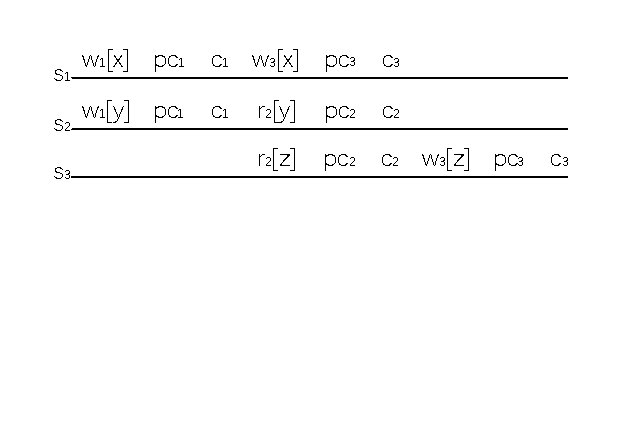
\includegraphics[scale=1]{figure/schedule_strict.pdf}}
  \caption{A strict and serializabile schedule ${H_1}$}
  \label{fig:strict_example}
\end{figure}

\begin{figure}[htbp]
  \centerline{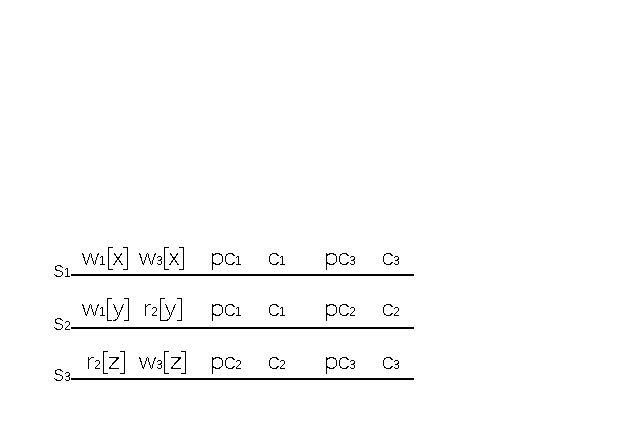
\includegraphics[scale=1]{figure/schedule_non_strict.pdf}}
  \caption{A non-strict but serializabile schedule ${H_2}$}
  \label{fig:non_strict_example}
\end{figure}

\begin{figure}[htbp]
  \centerline{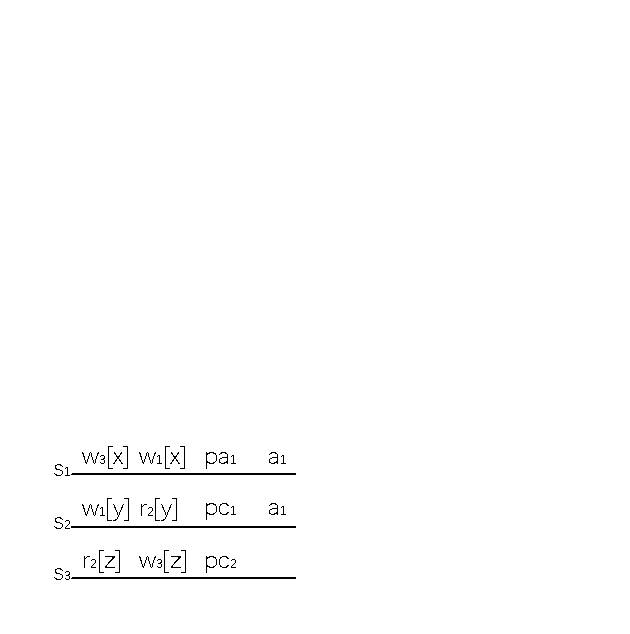
\includegraphics[scale=1]{figure/schedule_not_serializabile.pdf}}
  \caption{Schedule ${H_3}$, ${T_1}$ abort due to non-serializabile}
  \label{fig:schedule_abort_example}
\end{figure}

\begin{figure}[htbp]
  \centerline{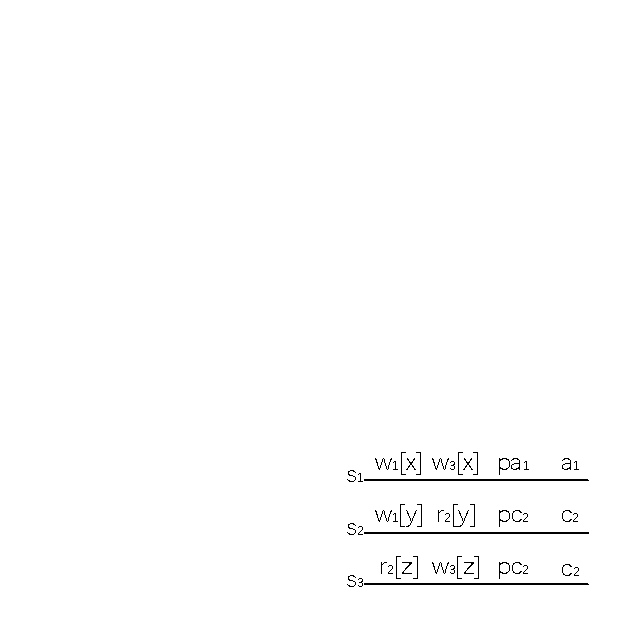
\includegraphics[scale=1]{figure/schedule_not_recoverable.pdf}}
  \caption{Schedule ${H_4}$, ${T_2}$ commit ahead ${T_1}$, non-recoverable anomaly}
  \label{fig:schedule_not_recoverable}
\end{figure}


As we can see, by violating strictness, ${H_2}$ in Figure~\ref{fig:non_strict_example} enables a higher degree of concurrency.
To realize such a schedule, ${T_1}$ must release its lock or mark it as violatable before it commits.

The commit of a transaction may involve a lot of work, especially when it is a distributed commit.
Strictness requires a transaction to hold locks until it finishes committing. In a distributed environment, the lock holding time will be substantially increased.
Our basic idea is to develop a serializable but non-strict scheduler for distributed transactions and shorten the lock holding time.

Relaxation on strictness will, on the other hand, complicate the logging mechanism.
In a traditional logging mechanism, the dependencies among transactions completely comply with the persisting order of their logs \cite{ELR:dewitt_implementation_1984}\cite{EfficientLocking:conf/vldb/KimuraGK12}.
This guarantees the recoverability of scheduling, which requires that a transaction can commit only if the transactions which it has read from commit. 
When strictness no longer holds, we need other tactics to preserve recoverability.

%When we extended the non-strict locking scheme to distributed transaction, transaction dependency maintaining is more complex.
%The serializable scheduler is a correct one if it can prevent abort.
%But when there are aborted transactions, it does not.
%To produce the correct log, the schedule must be both commit serializable and recoverable\cite{UnifyCR:journals/is/AlonsoVABASW94}.
%The scheduler need to maintain commit dependencies to guarantee serializability and recoverability when exploiting non-strictness.

\subsection{Lock Violation and Dependency Tracing}

Lock violation is a technique to enable non-strict schedules.
For lock violation to be correct, it should first preserve serializability.
Considering the non-strict schedule ${H_3}$ in Figure \ref{fig:schedule_abort_example},
it contains three data dependencies:

\begin{center}
${w_3[x] \rightarrow _s w_1[x]}$,
${w_1[y] \rightarrow _s r_2[y]}$
${r_2[z] \rightarrow _s w_3[z]}$
\end{center}

This leads to a circle ${T_1 \rightarrow T_2 \rightarrow T_3 \rightarrow T_1}$, making the schedule non-serializable.
${H_3}$ is not possible if we apply S2PL. It becomes possible if we perform lock violation -- it allows
${T_2}$ to read from uncommitted ${T_1}$, and ${T_1}$ to overwrite uncommitted ${T_3}$.
Therefore, to preserve serializability, we need to trace the data dependencies among transactions. 
If a lock violation is about to result in a dependency cycle, we can disable it.
For instance, we forbid ${T_2}$ from violating the lock of ${T_1}$.

In fact, lock violation can occur at two occasions in transaction processing.
We call them \emph{early lock violation} and \emph{late lock violation}.
Suppose ${H}$ is a schedule which is created by lock violation. We complement ${H}$  with the lock, unlock and lock violation operations,
so it looks as follows:
\begin{center}
  ${H = l_i[x] o_i[x]... vl_j[x] o_j[x]...  l_i[y] o_i[y]... ul_i[x] ... }$
\end{center}
In ${H}$, ${x}$, ${y}$ are separate records.
${T_i}$ first locks ${x}$ (i.e., $l_i[x]$).
Then, ${T_j}$ violates  ${T_i}$'s lock on ${x}$ (i.e., $vl_j[x]$).
Following that, ${T_i}$ locks ${y}$ and releases its lock on ${x}$ (i.e., $l_i[y]... ul_i[x]$).
If a lock violation, such as $vl_j[x]$, occurs before its victim transaction plays another lock, such as $l_i[y]$,
we call it an \emph{early lock violation}.
Otherwise, we call it a \emph{late lock violation}.

It was proven in \cite{a} that \emph{early lock violation} can lead to non-serializable schedules.
When using early lock violation, we have to trace all data dependencies to ensure that the dependency graph is acyclic.
In contrast, \emph{late lock violation} is safe, as it cannot make an acyclic dependency graph cyclic.
Our DLV chooses to perform late lock violation only.

%When ${T_1}$ abort for non-serializable, ${T_2}$ must cascade abort to avoid anomaly.
%Assume a lock violation scheduler creates schedule ${H_3}$.
%Not formally discussing, a lock violation operation is just as a transaction releases its lock and another later transaction acquire this lock.
%Then the schedule ${H_3}$ failed to comply with 2PL's two-phase principle.

%For a traditional locking CC scheme, transaction ${T_2}$ needs to wait for ${T_1}$'s release its lock until ${T_1}$ commit.
%This situation is like Figure~\ref{fig:strict_example}.
%Lock violation scheduler must guarantee the dependency graph has no circles.
%A transaction must trace commit dependencies if it violates locks of another conflict transaction operation.

Secondly, a schedule generated by lock violation must be recoverable.
In the schedule ${H_4}$ in Figure~\ref{fig:schedule_not_recoverable}, due to lock violation,
${T_2}$ reads  ${T_1}$'s write and commits before ${T_1}$.
%There is a danger dependency, ${w_1[y] \rightarrow_s r_2[y]}$ and ${T_2}$ 's commit is ahead ${T_1}$'s commit.
If ${T_1}$ decides to abort, it is no longer possible to reverse ${T_2}$.
As a result, schedule ${H_4}$ is not recoverable.
%If ${T_1}$ abort, then ${T_2}$ will return an error ${y}$ value.
To ensure recoverability, we need to trace the wr-dependencies among transactions, to ensure that the commit order complies with the wr-dependencies.



%This can be proved by formulating \emph{late lock violation} as 2PL proving.


Suppose there is a \emph{wr-dependency} from ${T_i}$ to ${T_j}$,
which is written as ${w_i[x] \rightarrow r_j[x]}$.
For recoverability, we must ensure that ${T_j}$ cannot commit if ${T_i}$ has not committed.
Traditional S2PL can guarantee this by releasing ${T_i}$'s locks after ${T_i}$ commit.
%Lock violating violates locking rule and ${T_j}$ can read ${T_i}$'s write on ${x}$ before ${T_i}$ commits.
In the case of lock violation, we trace the wr-dependencies among transactions and make sure that a 2PC scheduler obeys the following rules:
%Composite with 2PC protocol, we have the following rules:
\begin{enumerate}
  \item ${T_j}$'s RM can be prepared only if ${T_i}$ has committed;
  \label{rule:prepare}

  \item ${T_j}$'s TM can send out `commit' request only if ${T_i}$ has committed;
  \label{rule:commit}

  \item If ${T_i}$ aborts, ${T_j}$ must also abort too.
  \label{rule:abort}
\end{enumerate}

%By tracing dependencies after violating a lock, DLV schedule achieves both serializability and recoverability.

%Besides the consideration of correctness, other design considerations also arise in face of lock violation.
%One question is when to perform lock violation in 2PC.
%If we perform lock violation before the first phase of 2PC, it can shorten the lock holding time to the most extent.
%However, it may face more cascade aborts, which is a serious overhead.
%If we perform lock violation at the second phase of 2PC, its effects will be weakened.

\section{DLV implementation}
\label{sec:implement}

In this section, we introduce DLV implementation.
The following contents would include:
How DLV can avoid complex recovery algorithm and maintain the most limited amount of dependencies;
How DLV choose the proper time of enabling violation;
The wait-die policy of DLV use;
The pseudocode code description finally.

\subsection {In Memory Speculative Versions}

The non-strict scheduler needs more complex recovery algorithm to keep the correctness.
Take a schedule ${H_5}$ as an example,

\begin{center}
${H_5 = w_1[x]w_1[y]r_2[x]w_2[y]a_1a_2}$
\end{center}

If transaction ${T_1}$ abort, this cause cascade abort for recoverability.
Traditional database use undo log to process recovery transaction write operations.
Implementation undo log maybe a little bit tricky when exploiting non-strict.
A wrong recovery expand schedule of ${T_1}$ may be like ${exp(H_5)}$,
in which ${w^-_i[x]}$ means transaction ${T_i}$ undo its write on ${x}$.

\begin{center}
  ${exp(H_5) =  w_1[x]w_1[y]r_2[x]w_2[y]}$
  ${w^-_1[y]w^-_1[x]c_1w^-_2[y]c_2}$
\end{center}

Suppose the initial value of records ${x}$ and ${v}$ of are both 0.
The value of records ${x}$, ${y}$ and the undo log formatted after executing every operations in $exp(H)$ is shown in Table~\ref{tbl:x_y_vlues}.
Finally, after the execution of this schedule, both transaction ${T_1}$ and ${T_2}$ aborts.
The value of ${y}$ is 1, which the correct result should be the initial value 0.

\begin{table}[htb]
  \centering
  \begin{tabular}{|c|c|c|c|c|c|}
  \hline
operations & x &  y & undo   \\
  \hline
  \hline
  $w_1[x=1]$ & 1 & 0 & x=0  \\
  \hline
  $w_1[y=1]$ & 1 & 1 & y=0   \\
  \hline
  $r_2[x]$ & 1 & 1 &    \\
  \hline
  $w_2[y=2]$ & 1 & 2 & y=1  \\
  \hline
  $w^-_1[y=0]$ & 1 & 0 &   \\
  \hline
  $w^-_1[x=0]$ & 0 & 0 &   \\
  \hline

  $c_1$ & 0 & 0 &   \\
  \hline
  $w^-_2[y=1]$ & 0 & 1 &    \\
  \hline
  $c_2$ & 0 & 1 &  \\
  \hline
  \end{tabular}
\caption{x, y values, undo log after the execution of ${exp(H_5)}$}
\label{tbl:x_y_vlues}
\end{table}

To tackle this anomaly, recovery must use a more complex algorithm such as SOT\cite{UnifyCR:journals/is/AlonsoVABASW94}.
For schedule ${H_5}$, a correct recovery expandation may be:
\begin{center}
${exp^*(H_5) = w_1[x]w_1[y]r_2[x]w_2[y]w^-_2[y]c_2w^-_1[y]w^-_1[x]c_1}$
\end{center}
The schdeuler must recovery transaction by the reserve order of write operation.
If ${x}$ and ${y}$ is on the same database node and use \emph{late lock violation}, the recovery of a transaction is simple.
Because there is no partial failure, the transaction would commit in log order.
No additional work is needed when system recovery using traditional Aries algorithm\cite{ARIES:journals/tods/MohanHLPS92}.

However, if ${x}$ and ${y}$ are not located at the same node, this undo operation order is hard to accomplish because of partial failure.
When using \emph{early lock violation}, there are similar problems since transaction recovery must also undo transactional operations by reserve order.
To avoid this complexity, DLV maintains uncommitted speculative versions in memory and accepts no-steal policy when writing data.
No-steal policy need storage cannot write uncommitted data to permanent storages.
For most transactions would write a little data except the bulk loading ones and the modern database runs on a machine with large RAM, using no-steal policy to save memory is not necessary.
By no-steal and speculative versions, the database needs no undo log, transaction rollback and failure recovery would be more simple and efficient.
DLV 's speculative version implementation is a little similar with many multi-version concurrency control scheme.
The list is structured from the newest version to the oldest version and the last version of this list is the committed version.
Speculation versions are always stored in main memory and needs no persistence.
If a transaction would abort, it only needs to remove its write versions from speculative version list.

Previously, we have discussed that a \emph{ww} dependency does not affect recoverability.
\emph{Late lock violation}, since it has promised serializability, so it can ignore ${ww}$ and ${rw}$ dependencies and only trace ${wr}$ dependencies for recoverability.
Figure~\ref{fig:versions_example} show a series of schedule access on two contention rows, ${x}$, ${y}$.
The green rectangles are speculative versions and the red ones are committed versions.
Although there is ${ww}$ dependency ${w_6[x] \rightarrow w_4[x]}$.
The abort of $T_4$ does not cause ${T_6}$ cascade abort.
\begin{figure}[htbp]
  \centering
  \captionsetup[subfigure]{margin={0cm,0cm}}
  \subfloat[\small ${H_a = w_1[x_0]w_1[y_0]c_1w_2[x_1]w_3[x_2]w_3[y_1]w_4[x_3]}$]
  {
    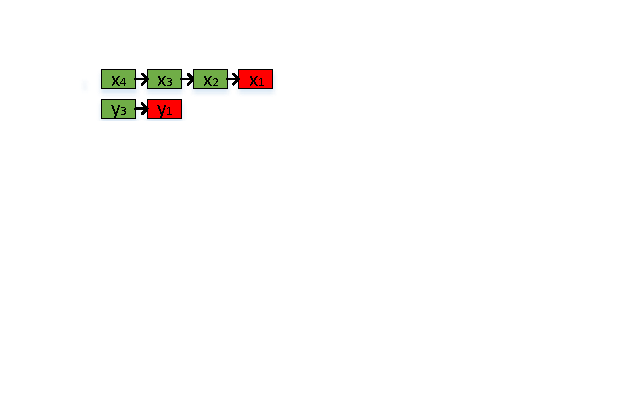
\includegraphics[scale=1.5] {figure/version1} \label{fig:versions_a}}
    \captionsetup[subfigure]{margin={0cm,0cm}
  }
  \subfloat[\small ${H_b = H_a c_2r_5[y_3]r_6[x_4]}$]
  {
    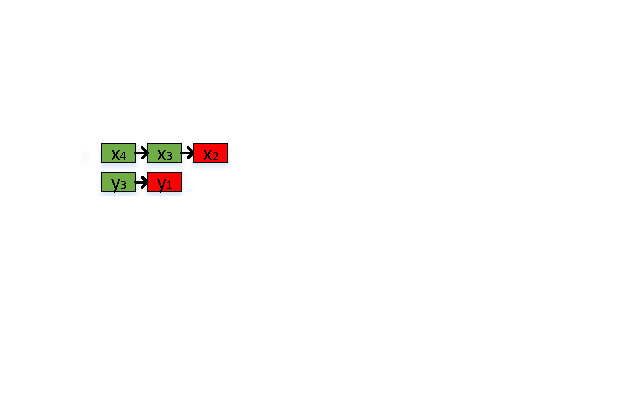
\includegraphics[scale=1.5]{figure/version2} \label{fig:versions_b}
  }
    \captionsetup[subfigure]{margin={0cm,0cm}
  }
  \subfloat[\small ${H_c = H_b a_3a_5}$]
  {
    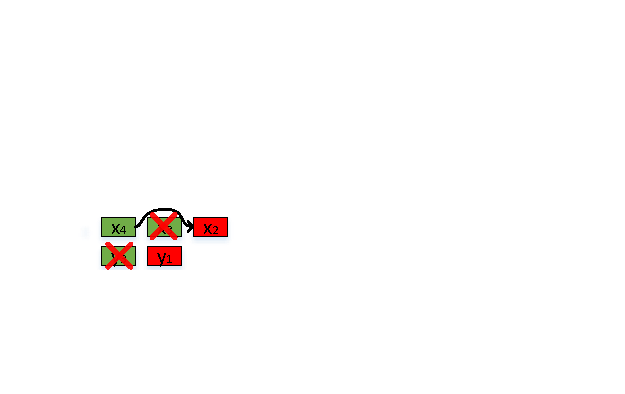
\includegraphics[scale=1.5] {figure/version3} \label{fig:versions_c}}
    \captionsetup[subfigure]{margin={0cm,0cm}}
    \subfloat[\small ${H_d = H_c c_4r_6[y_1]c_6}$]
      { 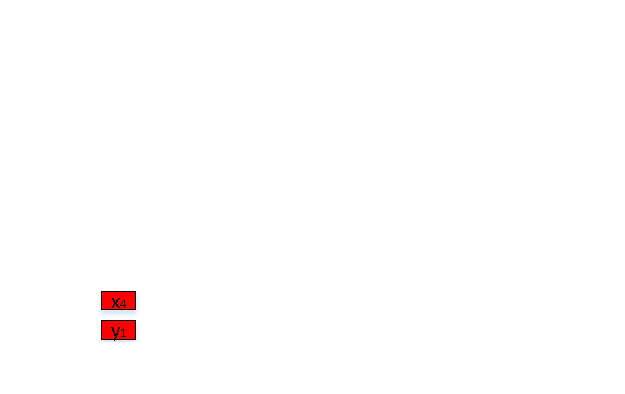
\includegraphics[scale=1.5]{figure/version4} \label{fig:versions_d}
  }
  \caption{speculative(green) and committed(red) versions,
  ${x_i}$ , ${y_i}$ express this version is from transaction transaction ${T_i}$'s write
}
\label{fig:versions_example}
\end{figure}

\subsection {Dynamic Decide Early or Late Violation}

\emph{DLV} exploit \emph{early lock violation}
when transaction is on going even preceding transaction request its (prepare) commit.

\emph{Early lock violation} can is more appropriate then \emph{late lock violation} when there are less cascade abort caused by non-deterministic abort.
\emph{Early lock violation} also need more dependency tracing costs.
Too many cascade abort can contributed to a lot of useless work.

We implementation \emph{late lock violation} by adding a message round trip to prevent deterministic abort when use lock violation.
This additional message flow shows in Algorithm~\ref{alg:speculate_phase}.
In Figure~\ref{fig:two_layers_architecture}, the message is show as dotted arrow lines.
Before an ${RM}$ decides to replicate its prepare log, it also sends a \emph{Ready} message to ${TM}$ and tells ${TM}$ it will prepare this transaction.
\emph{Ready} message shows that the ${RM}$ will prepare commit or prepare abort.
When the \emph{TM} collect all \emph{RM}s \emph{Ready} message, it sends \emph{Violate} messages to tells every \emph{RMs} make their locks are violative.
An interactive-transaction can combine these messages with the last operations and prepare requests in passing, as Figure~\ref{fig:transaction_interactive} shows.
So, the interactive transaction needs no dynamic decides the lock violation time.
Interactive transactions use ${DLV}$ would only work as \emph{late violation}.
We mainly focus on discuss one-shot transaction model here.
For a one-shot transaction, this message flow also takes less time than the overall message flow of 2PC because of no log replication time dealy.
Especially when all the ${RMs}$ and the ${TM}$ are located in LAN, there is no WAN message RTT.

DLV records transaction statistic information to decide use \emph{early lock violateion} or \emph{late lock violation}.
Assume at some point there are ${n}$ most recency ending (commit or abort) transactions ${T_1, T_2, ... T_n}$.
For any transaction ${T_i}$, ${T_i}$ would access 
${|S(i)|}$ shards, we record this collection of shards by:

${S(i) = \{s_1(i), s_2(i), ..., s_{|S(i)|}(i)\}}$.

A partial transaction ${t_{ij}, 1 \le j \le |S(i)|}$, is ${T_i}$'s transactional sequence operations working on shard ${s_j(i)}$.
We define following conceptions on partial transaction ${t_{ij}}$:

\emph{partial span time, ${\gamma (i, j)}$   :}
${t_{ij}}$'s \emph{partial span time} is from when ${t_{ij}}$ begin its first access operation  to its finish writing its final end log(commit or abort) on its shards.

\emph{partial max lock wait time, $\delta{i, j}$, :}
The maximum waiting time on a lock of all the locks ${t_{ij}}$ acquires on its shards.

\emph{partial prepare:}
${t_{ij}}$ successfully prepared to commit(enter phase1 of 2PL) but failed to commit finally on its shards.
We use function ${\eta(i, j)}$ to express wheathor ${t_{ij}}$ is partial prepare or not.
When ${t_{ij}}$ is partial prepare, ${\eta(i, j)}$ returns 1.
Otherwise, it returns 0.





DLV would choose \emph{early lock violation} if the following conditions  satisfied.
Otherwise, it would use \emph{late lock violation}.
\begin{center}
  ${
    {\frac
      {\sum_{i = 1}^{n} \sum_{j = 1}^{|S(i)|} \gamma(i, j)}
      {\sum_{i = 1}^{n} \sum_{j = 1}^{|S(i)|} \delta(i, j)} 
    }
    >
    p{\frac
      {\sum_{i = 1}^{n} \sum_{j = 1}^{|S(i)|}  \eta(i, j)}
      {\sum_{i = 1}^{n} {|S(i)|}} 
    }
  }$
\label{ine:condition}
\end{center}

In this inequality,  ${p}$ is constant coefficients.
The term on the lefthand side of the inequality can be considered the cost saved by lock violation and the right term is the cost of possible cascade abort. 

\subsection {Locking Violation and Maintain Commit Dependencies}
DLV use \emph{wait-die} protocol to avoid deadlock.
At the beginning of a transaction, the transaction uses the current timestamp to generate a transaction id.
The conflict transaction operations are queued base their transaction id's order.


\emph{DLV} use register and report\cite{HeckatonMVCC:journals/pvldb/LarsonBDFPZ11} to maintain dependencies.
Every transaction context stores an in dependency transaction(${in\_dn}$) number count to record how many transactions is the transaction depend on.
The transaction also records an out transaction set(${out\_set}$) attribute record the transactions depend on it.
When a transaction ${T}$ speculative read from ${S}$.
${T}$ registers dependency from ${S}$ by adding ${T}$ to ${out\_set}$ of ${S}$ and increase ${in\_dn}$ of ${T}$ by one.
These steps are described by line 4 - 7 in function READ in Algorithm \ref{alg:execution_phase}.
A transaction cannot prepare if it's ${in\_dn}$ value is greater than 0, which means some in dependency transaction does not commit yet.
If a transaction's ${in\_dn}$ value is less than 0, the transaction must abort because there is some in dependency abort cause a cascade abort.
Algorithm~\ref{alg:prepare_phase} shows how to prepare a transaction.
When a transaction commits, this transaction would traversal its ${out\_set}$ and decrease every transaction's ${in\_dn}$ by one, this is shown in line 6 - 11 of Algorithm \ref{alg:commit_phase} function.
If a transaction aborts, it may cause a cascade abort.
Line 2 of function CASCADE in Algorithm \ref{alg:commit_phase} shows the assign ${in\_dn}$ by a negative value when cascade abort.

\subsection{Pseudocode Description}

Algorithm~\ref{alg:execution_phase} shows the execution phase of a transaction.
Algorithm~\ref{alg:prepare_phase} shows the prepare phase of a transaction.
Algorithm~\ref{alg:commit_phase} shows the commit phase of a transaction.
Algorithm~\ref{alg:speculate_phase} shows the speculation phase of a transaction.
\begin{algorithm}[!h]

  \caption{Execution phase of transaction ${T}$. Read and write a key}

  \begin{algorithmic}[1]
  \Function{Read}{$T,key$}
      \State ${newest\_version \gets Head(Tuple(key).version\_list)}$
      \If {${newest\_version}$ is created by transaction ${S}$ \newline \textbf{and} ${key}$ is ICommit locked by ${S}$ }
        \If {${T \notin S.out\_set }$}
          \State ${S.out\_set \gets S.out\_set \cup T}$
          \State ${T.in\_dn \gets T.in\_dn + 1}$
        \EndIf
      \EndIf
      \If {${key}$ is \emph{write} locked by transaction ${S}$}
        \State ${S.wait \gets S.wait + 1}$
        \State wait lock till die
        \If {die}
            \State ${T.no\_da \gets }$ \textbf{False}
            \State \textbf{return} die error.
        \EndIf
      \EndIf
      \If {${key}$ is \emph{IAbort} locked by transaction ${S}$}
        \State wait lock this lock released
      \EndIf
      \State Lock(${T, key, Read}$)
      \State \textbf{return} ${key}$'s value.

  \EndFunction
  \label{func:read}
  \end{algorithmic}


  \begin{algorithmic}[1]
  \Function{Write}{$T,key, value$}
    \If {${key}$ is \emph{read} or \emph{write} locked}
      \If {${key}$ is \emph{write} locked by transaction ${S}$}
        \State ${S.wait \gets S.wait + 1}$
      \EndIf
      \State wait lock till die
      \If {die}
        \State ${T.no\_da \gets }$ \textbf{False}
        \State \textbf{return} die error.
      \EndIf
    \EndIf
    \State Lock(${T, key, Write}$)
    \State add a new version of ${key}$'s tuple, assign ${value}$
  \label{func:write}
  \EndFunction
  \end{algorithmic}
  \label{alg:execution_phase}
\end{algorithm}

\begin{algorithm}[!h]
  \caption{Prepare phase of transaction ${T}$}
  \begin{algorithmic}[1]
  \Function{Prepare}{$T$}
    \State wait if ${T.in\_dn > 0}$
    \If {${T.in\_dn < 0}$}
      \State response \emph{TM} message \emph{\{Prepare Abort\}}
    \ElsIf {$T.in\_dn = 0$}
      \State response \emph{TM} message \emph{\{Prepare Commit\}} \newline or \emph{\{Prepare Abort\}}
    \EndIf
  \EndFunction
  \end{algorithmic}
  \label{alg:prepare_phase}
\end{algorithm}

\begin{algorithm}[!h]
  \caption{Commit phase of transaction ${T}$, commit and (cascade)abort function}
  \begin{algorithmic}[1]
  \Function{Commit}{$T$}
    \State garbage collect old version in \newline ${Tuple(key).version\_list}$
    \For {$ key \in T.write\_set \cup T.read\_set$}
      \State Unlock(${T, key, Read/Write}$)
    \EndFor
    \For {${T_{out} \in T.out\_set}$}
      \State ${T_{out}.in\_dn \gets T_{out}.in\_dn - 1}$ \Comment{keep exactly once}
      \If ${T_{out}.in\_dn = 0}$
        \State report ${T_{out}.in\_dn = 0}$ \Comment{ stop waiting on function PREPARE line 2}
      \EndIf
    \EndFor
    \State response \emph{TM} message \emph{\{Commit ACK\}}
    \label{func:commit}
  \EndFunction
  \end{algorithmic}
  \begin{algorithmic}[1]
  \Function{ABORT}{$T$}
    \State \textbf{call} CASCADE(T)
    \For {$ key \in T.write\_set \cup T.read\_set$}
      \State Unlock(${T, key, Read/Write}$)
    \EndFor
    \State response \emph{TM} message \emph{\{Abort ACK\}}
    \label{func:abort}
  \EndFunction
  \end{algorithmic}
  \begin{algorithmic}[1]
    \Function{CASCADE}{$T$}
      \State ${T.in\_dn \gets -\infty }$
      \For {$ key \in T.write\_set$}
        \If {$key$ is ${ICommit}$ locked by ${T}$}
          \State ModifyLock($T, key, IAbort$)
        \EndIf
        \For {${version \in Tuple(key).version\_list}$}
          \If {${version}$ is created by ${T}$}
            \State remove ${version}$ from list
            \State \textbf{break}
          \EndIf
        \EndFor
      \EndFor
      \For {${T_{out} \in T.out\_set}$}
        \State \textbf{call} CASCADE(${T_{out}}$)
      \EndFor
      \label{func:cascade}
    \EndFunction
  \end{algorithmic}
  \label{alg:commit_phase}
\end{algorithm}

\begin{algorithm}[!h]

  \caption{Speculate phase. \
  \newline
  \emph{Ready} and \emph{Speculate} works on \emph{RM}.
  \newline
  \emph{TM} call \emph{Decide} send when \emph{TM} collects all \emph{RM}'s \emph{Ready} message.
  \newline
  \emph{msgs} is a collection of \emph{Ready} message which TM receives from all the \emph{RM}s.
  \newline
  ${\Theta}$ is a threshhold value to enable speculation.}
  \begin{algorithmic}[1]
  \Function{Ready}{$T$}
      \State response \emph{TM} message \newline \emph{\{Ready, ${wait \gets T.wait}$, ${non\_da \gets T.non\_da}$\}}
  \label{func:ready}
  \EndFunction
  \end{algorithmic}
  \begin{algorithmic}[1]
  \Function{Decide}{$T, msgs$}
    \If{${\forall m \in msgs}$, ${m.non\_da}$ is \textbf{True} \textbf{and} \newline
    ${\exists m \in msgs}$, ${m.wait > \Theta}$ }
      \State send all \emph{RM}s message \emph{\{Speculate\}}
    \EndIf
  \label{func:decide}
  \EndFunction
  \end{algorithmic}
  \begin{algorithmic}[1]
  \Function{Speculate}{$T$}
    \For {$ key \in T.read\_set$}
      \State Unlock($T, key, Read$)
    \EndFor
    \For {$ key \in T.write\_set$}
      \If {$key$ is ${Write}$ locked by ${T}$}
        \State ModifyLock($T, key, ICommit$)
      \EndIf
    \EndFor
  \label{func:speculate}
  \EndFunction
  \end{algorithmic}
  \label{alg:speculate_phase}
\end{algorithm}

\section{Experiments and Evaluations}
\label{sec:experiments}
We develop a replicated distributed DBMS demo and evaluate the performance of \emph{DLV}.
As a comparison with \emph{DLV}, we also implement S2PL wait die(S2PL) scheme, CLV optimize both violate at the 1st phase(CLV1P) and 2nd phase(CLV2P).

\subsection{Experiments Setting}
Our experiments performed on a cluster of 12 Aliyun ecs.g6.large server.
Each server has 2 virtual CPU with 2.5GHz clock speed, 8GB RAM, runs Ubuntu 18.04.
The data is partitioned by 4 shards, each shard has 3 replicas which is replicated across 3 AZs, which is located at Heyuan, Hangzhou and Huhehot.
Every AZ has a full data copy of each shard.
The internal network bandwidth of each AZ is 1Gbps.
We choose a modifies version TPCC and YCSB workload.
All the transactions are distributed transactions.
The TPCC data is sharded by the warehouse id.
The Item table is replicated to all shards.
Each transaction will retry after 3 seconds if it aborts for violation serializability.
The evaluation both tested on both scattered (leader) mode and gathered (leader) mode.
In gathered mode, all of the replica leaders are located in the same AZes.
In scattered mode, the replica leaders are not located in the same AZes.

\subsection{TPCC Performance Evaluation}
Figure \ref{fig:new_order_add_terminal_gathered} shows the NewOrder performance of when adding terminal numbers of each node in the gathered  mode and scattered mode.

Figure \ref{fig:new_order_add_warehouse_gathered},
Figure \ref{fig:payment_add_warehouse_gathered} shows
the performance of different warehouse numbers.


\begin{figure}[htbp]
  \centering
  \captionsetup[subfigure]{margin={0cm,0cm}}
  \subfloat[NewOrder TPM]
      { 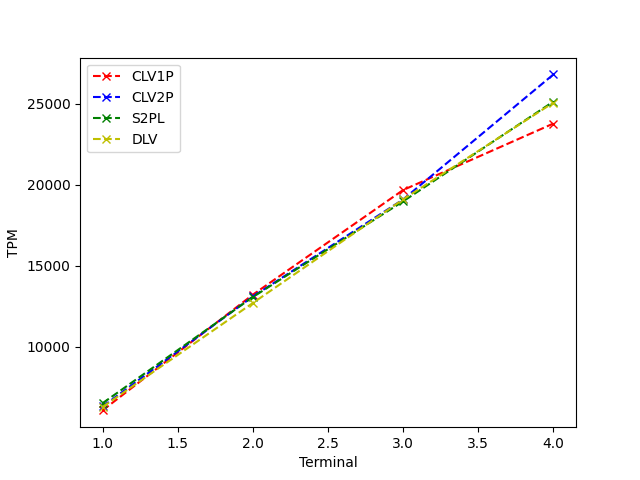
\includegraphics[scale=0.25] {figure/plot_tpcc_neworder_add_Terminal_gather_tpm} \label{fig:new_order_add_terminal_gathered:tpm}}
  \captionsetup[subfigure]{margin={0cm,0cm}}
  \subfloat[NewOrder abort]
      { 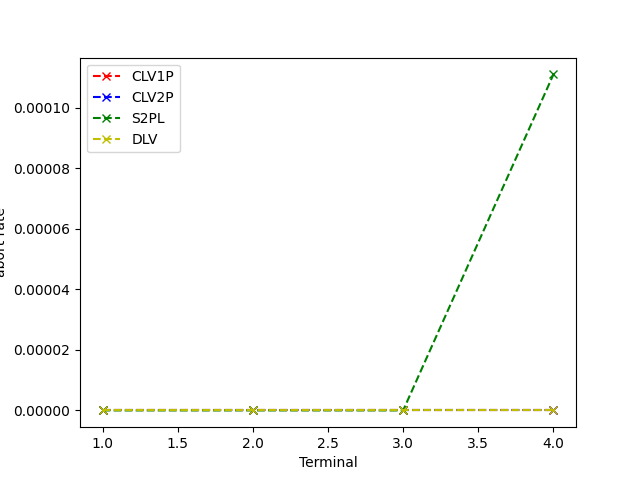
\includegraphics[scale=0.25]{figure/plot_tpcc_neworder_add_Terminal_gather_abort} \label{fig:new_order_add_terminal_gathered:abort}}
  \captionsetup[subfigure]{margin={0cm,0cm}}
\caption{throughput and abort rate of
different terminal number of each node
when running TPCC NewOrder transactions in gathered mode(TODO .. need more terminals, 4 is too small)}
\label{fig:new_order_add_terminal_gathered}
\end{figure}


\begin{figure}[htbp]
  \centering
  \captionsetup[subfigure]{margin={0cm,0cm}}
  \subfloat[NewOrder TPM]
      { 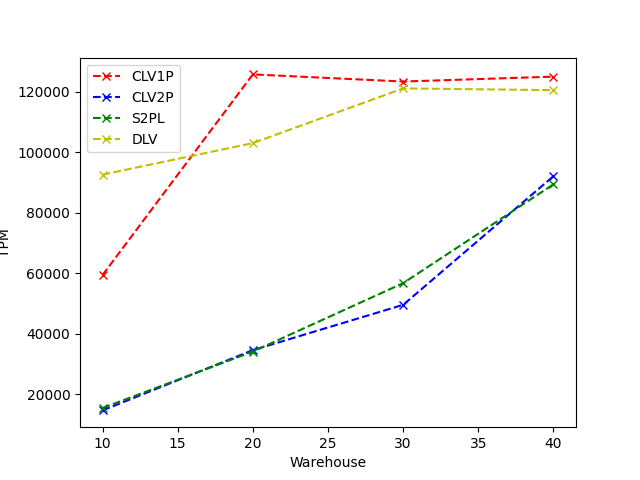
\includegraphics[scale=0.25] {figure/plot_tpcc_neworder_add_Warehouse_gather_tpm} \label{fig:new_order_add_warehouse_gathered:tpm}}
  \captionsetup[subfigure]{margin={0cm,0cm}}
  \subfloat[NewOrder abort]
      { 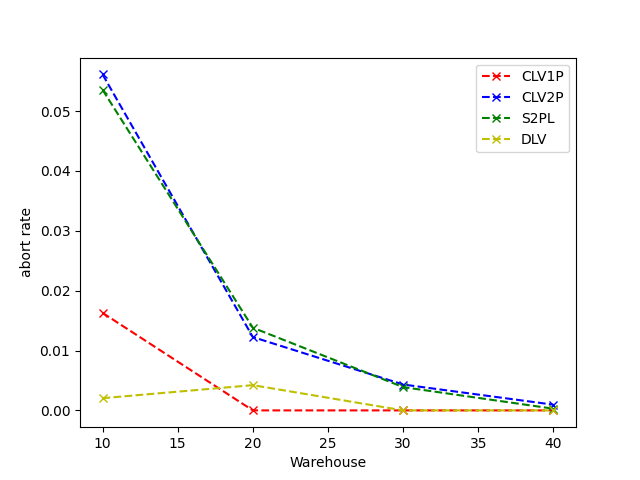
\includegraphics[scale=0.25]{figure/plot_tpcc_neworder_add_Warehouse_gather_abort} \label{fig:new_order_add_warehouse_gathered:abort}}
  \captionsetup[subfigure]{margin={0cm,0cm}}
\caption{throughput and abort rate of
different warehouse number
when running TPCC NewOrder transactions in gathered mode}
\label{fig:new_order_add_warehouse_gathered}
\end{figure}

\begin{figure}[htbp]
  \centering
  \captionsetup[subfigure]{margin={0cm,0cm}}
  \subfloat[Payment TPM]
      { 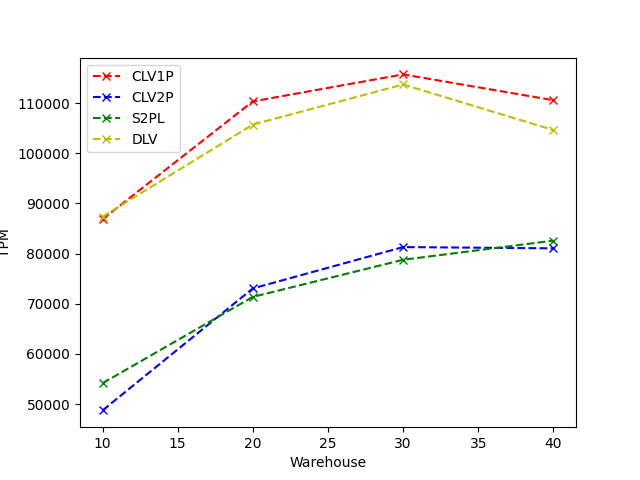
\includegraphics[scale=0.25] {figure/plot_tpcc_payment_add_Warehouse_gather_tpm} \label{fig:payment_add_warehouse_gathered:tpm}}
  \captionsetup[subfigure]{margin={0cm,0cm}}
  \subfloat[Payment abort]
      { 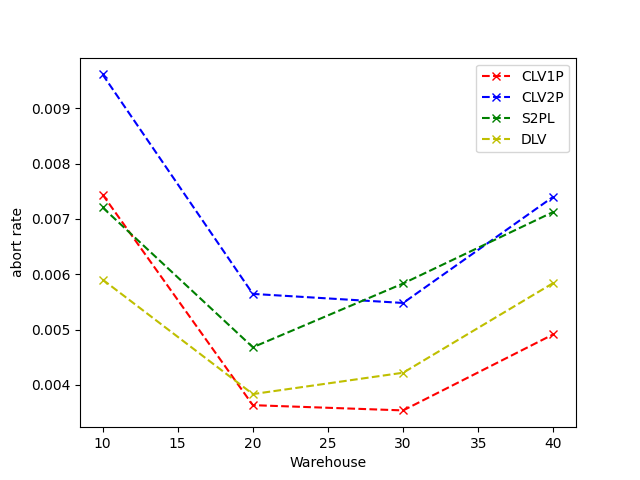
\includegraphics[scale=0.25]{figure/plot_tpcc_payment_add_Warehouse_gather_abort} \label{fig:payment_add_warehouse_gathered:abort}}
  \captionsetup[subfigure]{margin={0cm,0cm}}
\caption{throughput and abort rate of
different warehouse number
when running TPCC Payment transactions in gathered mode}
\label{fig:payment_add_warehouse_gathered}
\end{figure}



\begin{figure}[htbp]
  \centering
  \captionsetup[subfigure]{margin={0cm,0cm}}
  \subfloat[NewOrder TPM]
      { 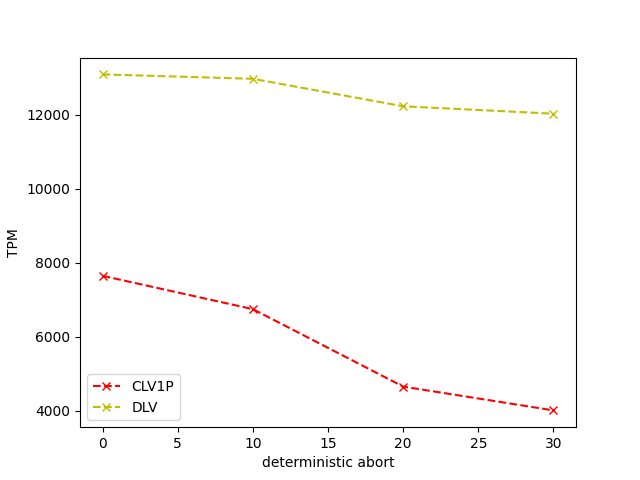
\includegraphics[scale=0.25] {figure/plot_tpcc_neworder_add_NonExist_gather_tpm} \label{fig:plot_tpcc_neworder_add_NonExist_gather_abort:tpm}}
  \captionsetup[subfigure]{margin={0cm,0cm}}
  \subfloat[NewOrder abort]
      { 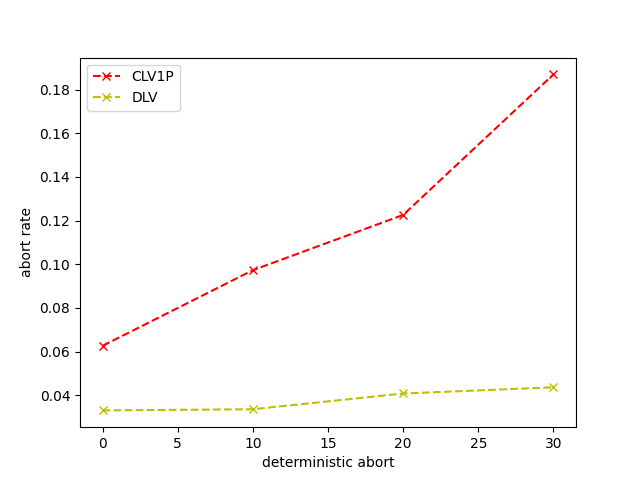
\includegraphics[scale=0.25]{figure/plot_tpcc_neworder_add_NonExist_gather_abort} \label{fig:plot_tpcc_neworder_add_NonExist_gather_abort:abort}}
  \captionsetup[subfigure]{margin={0cm,0cm}}
\caption{throughput and abort rate of
different possible cascade abort rate,
when running TPCC NewOrder transactions in gathered mode}
\label{fig:plot_tpcc_neworder_add_NonExist_gather_abort}
\end{figure}



\begin{figure}[htbp]
  \centering
  \captionsetup[subfigure]{margin={0cm,0cm}}
  \subfloat[NewOrder TPM]
      { 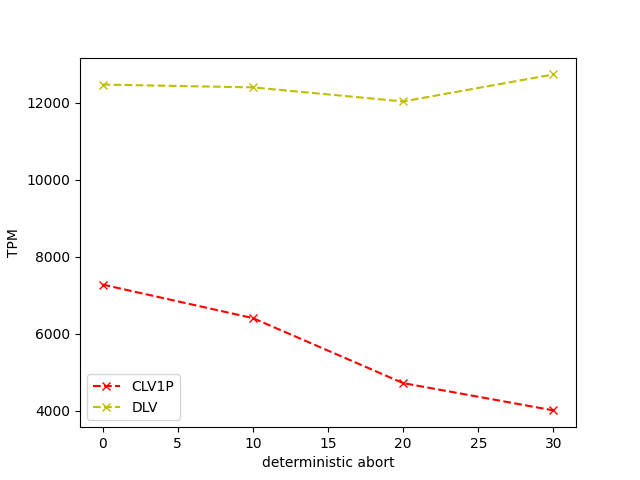
\includegraphics[scale=0.25] {figure/plot_tpcc_neworder_add_NonExist_scatter_tpm} \label{fig:plot_tpcc_neworder_add_NonExist_scatter:tpm}}
  \captionsetup[subfigure]{margin={0cm,0cm}}
  \subfloat[NewOrder abort]
      { 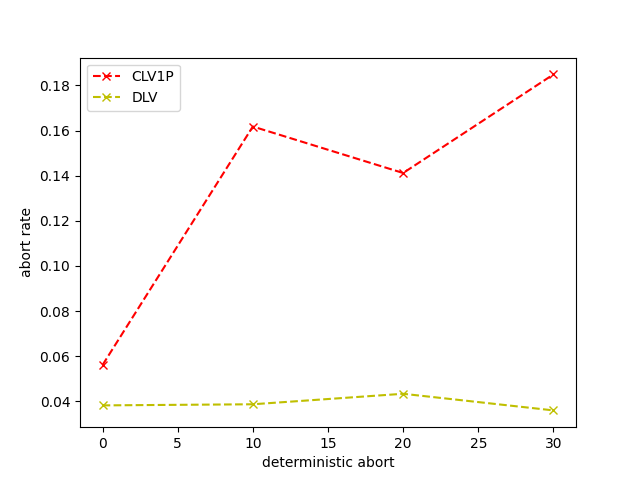
\includegraphics[scale=0.25]{figure/plot_tpcc_neworder_add_NonExist_scatter_abort} \label{fig:plot_tpcc_neworder_add_NonExist_scatter:abort}}
  \captionsetup[subfigure]{margin={0cm,0cm}}
\caption{throughput and abort rate of
different possible cascade abort rate,
when running TPCC NewOrder transactions in scattered mode
}
\label{fig:plot_tpcc_neworder_add_NonExist_scatter}
\end{figure}

\subsection{YCSB Performance Evaluation}

\begin{figure}[htbp]
  \centering
  \captionsetup[subfigure]{margin={0cm,0cm}}
  \subfloat[YCSB TPM]
      { 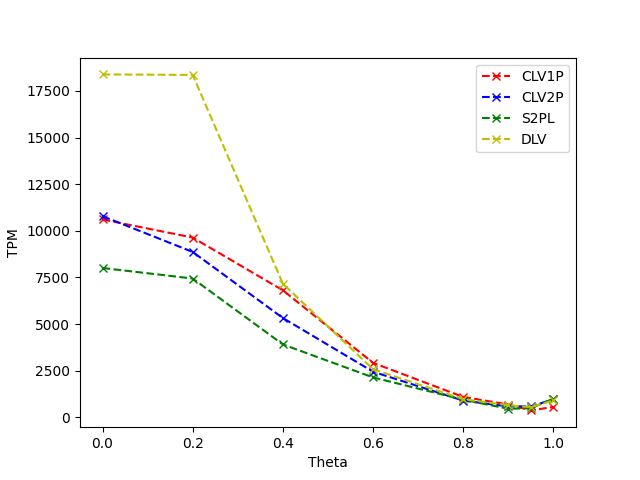
\includegraphics[scale=0.25] {figure/plot_ycsb_add_Theta_gather_tpm} \label{fig:ycsb_add_theta_gathered:tpm}}
  \captionsetup[subfigure]{margin={0cm,0cm}}
  \subfloat[YCSB abort]
      { 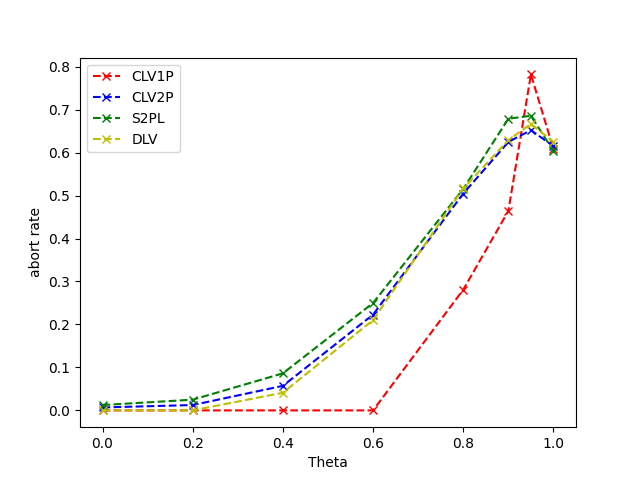
\includegraphics[scale=0.25]{figure/plot_ycsb_add_Theta_gather_abort} \label{fig:ycsb_add_theta_gathered:abort}}
  \captionsetup[subfigure]{margin={0cm,0cm}}
\caption{throughput and abort rate of
different warehouse number
when running YCSB transactions in gathered mode}
\label{fig:ycsb_add_theta_gathered}
\end{figure}

\begin{figure}[htbp]
  \centering
  \captionsetup[subfigure]{margin={0cm,0cm}}
  \subfloat[YCSB TPM]
      { 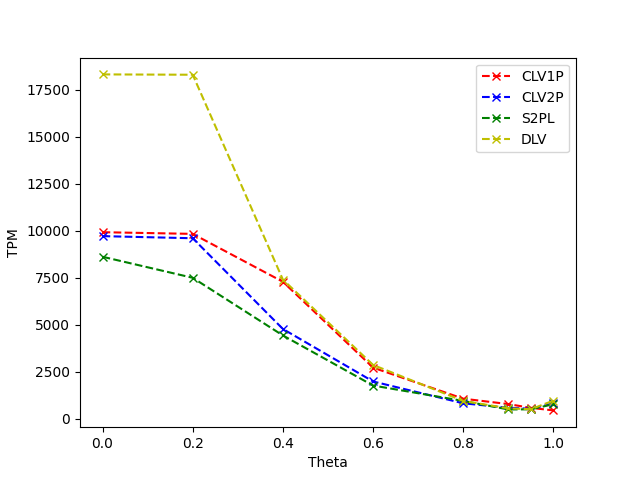
\includegraphics[scale=0.25] {figure/plot_ycsb_add_Theta_scatter_tpm} \label{fig:ycsb_add_theta_scattered:tpm}}
  \captionsetup[subfigure]{margin={0cm,0cm}}
  \subfloat[YCSB abort]
      { 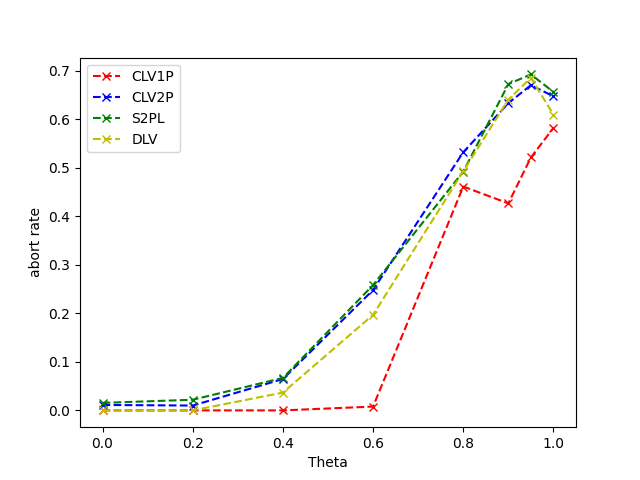
\includegraphics[scale=0.25]{figure/plot_ycsb_add_Theta_scatter_abort} \label{fig:ycsb_add_theta_scattered:abort}}
  \captionsetup[subfigure]{margin={0cm,0cm}}
\caption{throughput and abort rate of
different warehouse number
when running YCSB transactions in scattered mode}
\label{fig:ycsb_add_theta_scattered}
\end{figure}



\section{Conclution}
\label{sec:conclution}
We extend $CLV$ to distributed transaction and evaluate its performance on a geo-replicated environment.
Our distributed version ${CLV}$, i.e. ${DLV}$, can dynamically decide to violate lock at the most suitable time.
${DLV}$ merge many discrete waits at transaction running time into one final wait when commit.
According to our evaluation, ${DLV}$ can improve performance of contention workload for shortening critical path.
${DLV}$ can adapt to different workloads.
It minimize unnecessary dependency tracing cost and cascade abort penalty against previous work.






\bibliographystyle{reference/IEEEtran}
\bibliography{reference/IEEEexample}


\end{document}

